\documentclass[tikz,border=7pt]{standalone}
\usepackage{libertinus}
\usepackage{amsmath}
\usetikzlibrary{
  arrows.meta,
  backgrounds,
  calc,
  decorations.markings,
  fit,
  positioning
}

\definecolor{accent}{RGB}{38,103,115}
\definecolor{softgray}{RGB}{244,245,246}
\definecolor{midgray}{RGB}{123,128,132}

\tikzset{
  >={Latex[length=2.2mm,width=1.5mm]},
  flow/.style={-Latex,semithick,draw=black!72},
  accent flow/.style={-Latex,semithick,draw=accent},
  box/.style={
    draw=black!68,
    fill=softgray,
    rounded corners=1.2pt,
    align=center,
    inner xsep=5pt,
    inner ysep=4pt
  },
  accent box/.style={
    draw=accent,
    fill=accent!8,
    rounded corners=1.2pt,
    align=center,
    inner xsep=5pt,
    inner ysep=4pt
  },
  point/.style={circle,draw=black!75,fill=white,inner sep=1.7pt},
  accent point/.style={circle,draw=accent,fill=accent!10,inner sep=1.7pt},
  tinylabel/.style={font=\scriptsize,align=center},
  smalllabel/.style={font=\small,align=center},
  panel/.style={draw=black!28,rounded corners=2pt,inner sep=6pt}
}

\begin{document}
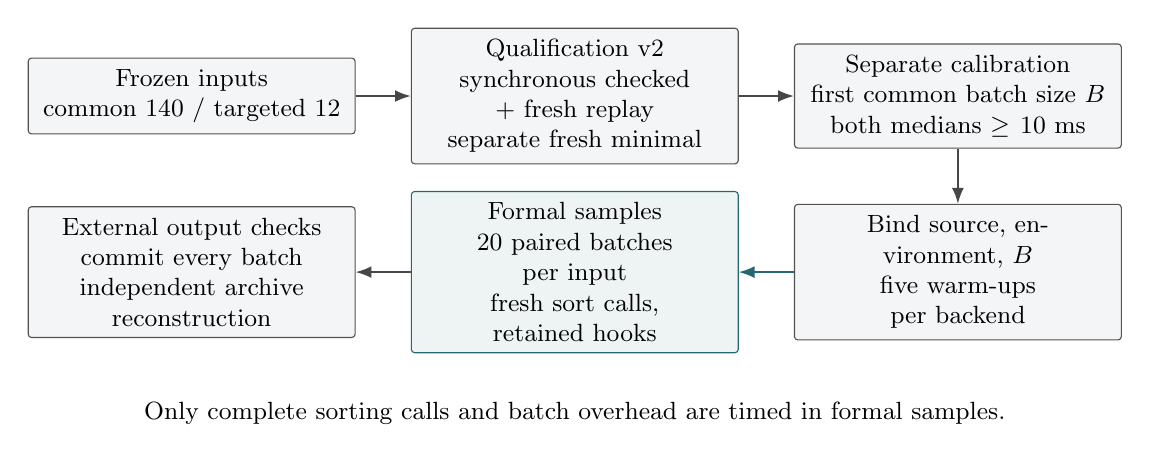
\begin{tikzpicture}[font=\small,node distance=7mm and 7mm]
\node[box,text width=3.8cm] (inputs) {Frozen inputs\\common 140 / targeted 12};
\node[box,text width=3.8cm,right=of inputs] (qual) {Qualification v2\\synchronous checked + fresh replay\\separate fresh minimal};
\node[box,text width=3.8cm,right=of qual] (cal) {Separate calibration\\first common batch size $B$\\both medians $\geq10$ ms};
\node[box,text width=3.8cm,below=of cal] (gate) {Bind source, environment, $B$\\five warm-ups per backend};
\node[accent box,text width=3.8cm,left=of gate] (sample) {Formal samples\\20 paired batches per input\\fresh sort calls, retained hooks};
\node[box,text width=3.8cm,left=of sample] (check) {External output checks\\commit every batch\\independent archive reconstruction};
\draw[flow] (inputs)--(qual); \draw[flow] (qual)--(cal);
\draw[flow] (cal)--(gate); \draw[accent flow] (gate)--(sample);
\draw[flow] (sample)--(check);
\node[smalllabel,below=5mm of sample] {Only complete sorting calls and batch overhead are timed in formal samples.};
\end{tikzpicture}
\end{document}
